% Link: https://tex.stackexchange.com/questions/127375/replicate-the-fourier-transform-time-frequency-domains-correspondence-illustrati
\documentclass[border=5mm]{standalone}
\usepackage{pgfplots}
\pgfplotsset{compat=1.8}

\begin{document}
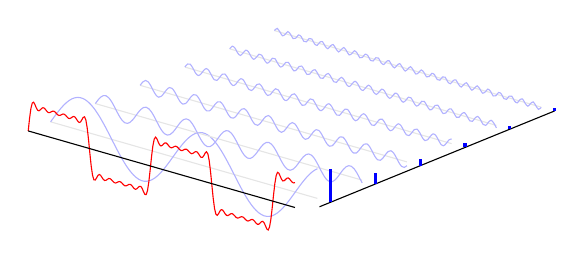
\begin{tikzpicture}
\begin{axis}[
    set layers=standard,
    domain=0:10,
    samples y=1,
    view={40}{20},
    hide axis,
    unit vector ratio*=1 2 1,
    xtick=\empty, ytick=\empty, ztick=\empty,
    clip=false
]
\def\sumcurve{0}
\pgfplotsinvokeforeach{0.5,1.5,...,5.5}{
    \draw [on layer=background, gray!20] (axis cs:0,#1,0) -- (axis cs:10,#1,0);
    \addplot3 [on layer=main, blue!30, smooth, samples=101] (x,#1,{sin(#1*x*(157))/(#1*2)});

    \addplot3 [on layer=axis foreground, very thick, blue,ycomb, samples=2] (10.5,#1,{1/(#1*2)});
    \xdef\sumcurve{\sumcurve + sin(#1*x*(157))/(#1*2)}
}
\addplot3 [red, samples=200] (x,0,{\sumcurve});

\draw [on layer=axis foreground]  (axis cs:0,0,0) -- (axis cs:10,0,0);
\draw (axis cs:10.5,0.25,0) -- (axis cs:10.5,5.5,0);
\end{axis}
\end{tikzpicture}
\end{document}
